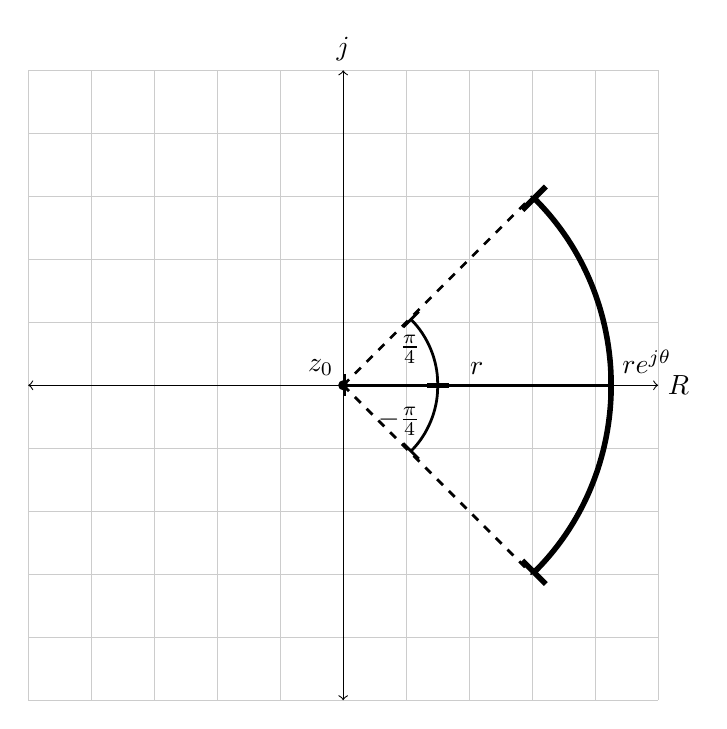
\begin{tikzpicture}[scale=0.8]
    \draw[thin,gray!40] (-5,-5) grid (5,5);
    \draw[<->] (-5,0)--(5,0) node[right] {$R$};
    \draw[<->] (0,-5)--(0,5) node[above]{$j$};
    \draw[line width=2pt,black,|-|] (3,-3) arc (-45:45:4.2426) node [midway,anchor=south west]{$re^{j\theta}$};
    \draw[line width=1pt,black,|-|] (1.5,0) arc (0:45:1.5) node [midway, left]{$\frac{\pi}{4}$};
    \draw[line width=1pt,black,|-|] (1.5,0) arc (0:-45:1.5) node [midway, left]{$-\frac{\pi}{4}$};
    \draw[fill=black] (0,0) circle(2pt) node[anchor=south east]{$z_0$};
    \draw[line width=1pt,black,dashed] (0,0)--(3,3);
    \draw[line width=1pt,black,dashed] (0,0)--(3,-3);
    \draw[line width=1pt,black,|-|] (0,0)--(4.2426,0) node[midway,above,sloped]{$r$};

  
\end{tikzpicture}
\caption{Arco en el plano complejo de centro $z_0$}